\documentclass[10pt]{beamer}
\usepackage[utf8]{inputenc}
\usepackage[T1]{fontenc}

\usetheme{acme}

\title[example]{Example ACME Beamer Slides}
\date{}
\author{Charlie Stuart }

\begin{document}

\begin{frame}[plain]
\titlepage
\end{frame}

\section{basiclatex}
\subsection{text.txt}
\begin{frame}
	\frametitle{Text On A Slide}

	This first section covers the basics in LaTeX that I use the most and
	require the least amount of styling.

	Here is an example pararaph.
	Just plain text.
	Nothing special.

	Lorem ipsum dolor sit amet, consectetur adipiscing elit.
	Integer imperdiet, leo nec posuere placerat, dolor leo pulvinar erat, non
	semper diam arcu molestie nulla.
	Donec non libero nec ante pharetra molestie.
	Praesent mollis, velit sit amet varius feugiat, massa enim auctor arcu,
	eget venenatis urna nunc eget lorem. Nunc rutrum quam sed volutpat blandit.
	Aliquam erat volutpat. Donec pretium tellus quis magna euismod, ac porttitor
	tortor placerat.
	Quisque eget risus a mauris pharetra sodales eu vitae diam.
	Ut vitae tristique felis.
	Nam blandit, dolor et lobortis imperdiet, sem erat mattis mi, non maximus
	justo ante eu diam.
\end{frame}

\subsection{tabular.txt}
\begin{frame}
	\frametitle{A Table}

	\begin{tabular}{| l l |}
	\hline
	\textbf{Column 1} & \textbf{Column 2} \\
	\hline
	Row 1 & Row 1 \\
	Row 2 & Row 2 \\
	Row 3 & Row 3 \\
	\hline
	\end{tabular}
\end{frame}

\subsection{itemenum.txt}
\begin{frame}
	\frametitle{Itemize and Enumerate}

	\begin{itemize}
	\item Item A
	\item Item B
	\item Item C
	\end{itemize}

	\begin{enumerate}
	\item Enumerate One
	\item Enumerate Two
	\item Enumerate Three
	\end{enumerate}
\end{frame}

\subsection{equationfig.txt}
\begin{frame}
	\frametitle{Equation Figure}


	\begin{figure}
		\[ \sum_{i=0}^n i =  \frac{n(n-1)}{2} \]
		\caption{Arithmetic Series}
	\end{figure}
\end{frame}

\subsection{image.png}
\begin{frame}
	\frametitle{An Image}
	\framesubtitle{Of The Title Frame}
	
	\begin{center}
	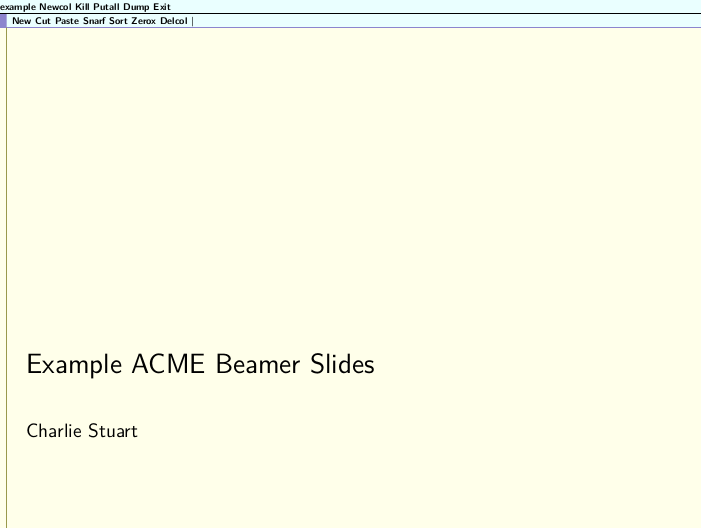
\includegraphics[scale=0.5]{example.png}
	\end{center}
\end{frame}


\section{gettingfancy}
\subsection{theorem.txt}

\begin{frame}[<+->]
	\frametitle{A Theorem}
	\framesubtitle{Taken From The Beamer User Guide}

	\begin{theorem}
		$A = B$.
	\end{theorem}
	\begin{proof}
		\begin{itemize}
		\item Clearly, $A = C$.
		\item As shown earlier, $C = B$.
		\item<3-> Thus $A = B$.
		\end{itemize}
	\end{proof}
\end{frame}

\end{document}
